
%Copyright (C) 2016 by Krishneel@JSK Lab, The University of Tokyo

\documentclass{standalone}
\usepackage{footnote}
\usepackage{hyperref}
\usepackage{graphicx}

\begin{document}

\subsection{Software}

The softwares are developed on ROS environment which includes motion planning, visual perception and virtual simulation. The simulation environment was developed on Gazebo simulator \footnote{\url{https://github.com/start-jsk/jsk_mbzirc}}. We used this simulator for planning our stretegy and for customization of our hardwares and softwares. The visual perception node involves target (heliport) localization on the moving vehicle, planning our efficient approaching and landing stretegy based on the motion of both the UAV and the vehicle. Since we use Nvidia TX1 embedded processor for fast computations on GPU, our algorithms for \textit{task 1} and \textit{task 3} are developed in CUDA-C, C/C++ and Python. 

% \begin{figure}[t]
%   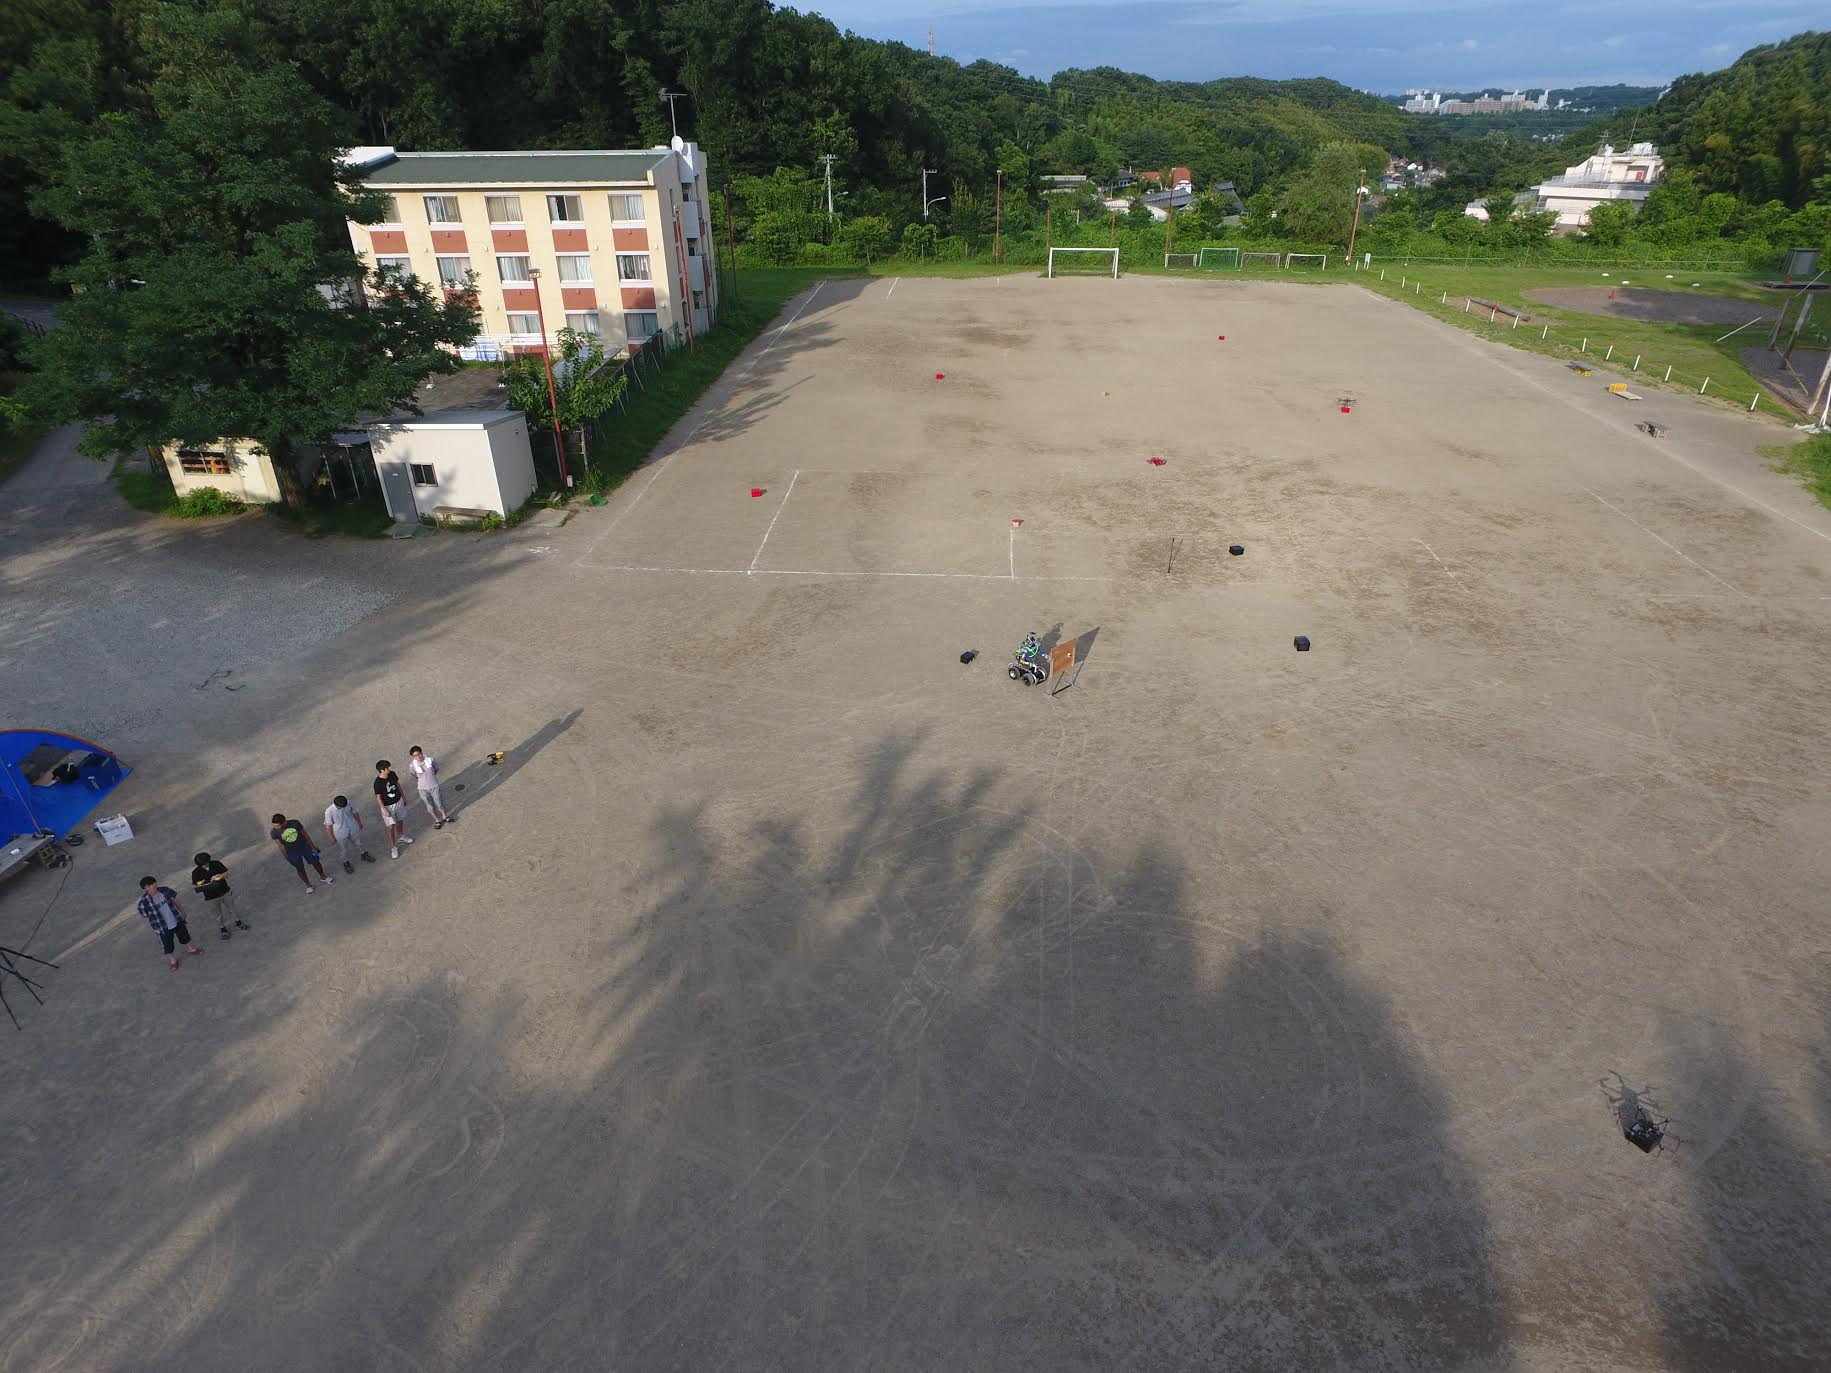
\includegraphics[width=\columnwidth, trim={2cm 5cm 3cm 7cm},clip]{sections/task1/images/testbed}
%   \caption{Testbed for outdoor testing in Hachioji, Tokyo, Japan}
% \end{figure}


\subsection{General Approach}

%\textbf{Vehicle And Heliport Detection}: 
We use the heliport model to train a linear classifier for detection of landing region. Since heliport model will be consistent it can be used as a priori for learning. Once the heliport is detected, a visual object tracker running at real time onboard is autonomously initalized to start tracking the target region. We use a robust tracking algorithm with efficient tracking drift compensation algorithm to avoid lost of target when the uav is in motion. Moreover our visual tracking algorithm is able to recover the target even if its completely out of view.

Once the target is localized, the UAV uses this information to navigate towards the target. 


\subsection{Future Works}
The future work on hardware platform for task 1 includes the design of landing gear which enables to attach to a moving heliport. The sturdy and light protector of UAV is another issue to avoid the crash while hitting to the truck.

The future work on software for task 1 involves the vision based egomotion estimation which is more robust than GPS based localization. With the stable flight platform, the testing the software associated with motion tracking which is developed on the simulation system will be operated on the actual UAV. Considering the challenges on the outdoor environment such as abrupt changes in image space, winds speeds etc., we believe that we will have to improve our current landing stretegy in the real world. 

\end{document}
